
Sile koje djeluju na projektil su u letu su aerodinamičke, pogonske sile i 
gravitaciona sila. Ove sile se mogu razložiti po osama kooridnatnog sistema vezanog 
za tijelo. 
\section{Aerodinamičke sile}
Aerodinamička sila je posljedica djelovanja pritiska okolnog fluida na tijelo u pokretu. 
Aerodinamička sila se može razložiti na tri komponente koje su definisane u nastavku:
\begin{itemize}
    \item \textbf{Uzgon}- Uzgon je komponenta rezultantne aerodinamičke sile 
    koja je normalna na relativno kretanje vjetra.
    \item \textbf{Otpor}- Otpor je komponenta rezultantne aerodinamičke sile 
    koja je paralelna relativnom kretanju vjetra.
    \item \textbf{Bočna sila}- Bočna sila je komponenta rezultantne aerodinamičke sile 
    koja je normalna na uzogn i otpor. 
\end{itemize}
Ovdje se posmatraju projektili koji se zakreću da bi skrenuli(skid to turn) i 
kod takvih projektila aerodinamičke sile su date sa:
\begin{equation}
   \text{Uzgon} \quad R_x=C_xqS
   \label{eq:a1}
\end{equation}
\begin{equation}
    \text{Otpor} \quad R_z=C_zqS
    \label{eq:a2}
\end{equation}
\begin{equation}
    \text{Bočna sila} \quad R_y=C_yqS
    \label{eq:a3}
\end{equation}
,gdje su $C_x,C_y$ i $C_z$ aerodinamički koeficijenti, $q$ dinamički pritisak slobodnog strujanaja
u tački daleko od objekta i iznosi $q=\frac{1}{2}\rho v^2$, $S$ je referentna površina i 
$v$ je brzina vazduha, $\rho$ predstavlja atmosferski pritisak.
\\
U opštem slučaju koeficijenti aerodinamičkih sila su funkcije varijabli stanja pa se može
napisati:
\begin{equation}
    C_x=C_x(\alpha ,\beta, M,q,\delta_v,\delta_P,\delta_e)
\end{equation}
,gdje je $M$ Mahov broj- odnos tekuće brzine i brzine zvuka, $\alpha$ napadni ugao i 
$\beta$ ugao klizanja. Slično tako vrijedi:
\begin{equation}
    C_z=C_z(\alpha ,\beta, M,q,\delta_v,\delta_P,\delta_e)
\end{equation}
Uglovi $\alpha, \beta$ i $\gamma$ su prikazani na slici \ref{fig:angles} i definisani su sa:
\begin{equation}
    \alpha=arctg(w/u)
\end{equation}
\begin{equation}
    \beta=\arcsin(v/v_m)
\end{equation}
\begin{figure}[h!]
    \centering
    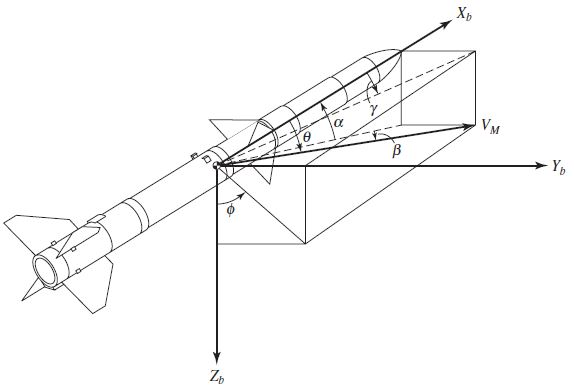
\includegraphics[scale=0.7]{angles.JPG}
    \caption{Ugaone veze}
    \label{fig:angles}
\end{figure}
Razvojem u Taylorov red i odbacivanjem viših članova dobija se aproksimacija 
aerodinamičkih koeficijenata:
\begin{equation}
    C_x=C_{x_0}+C_{x_\alpha}|\alpha|+C_{x_\alpha^2}\alpha^2+C_{x_\beta}|\beta|+
    C_{x_\beta^2}\beta^2+C_{x_\alpha \beta}|\alpha||\beta|
\end{equation}
\begin{equation}
    C_z=C_{z_0}+C_{z_\alpha}|\alpha|+C_{z_\alpha^2}\alpha^2+C_{z_\beta}|\beta|+
    C_{z_\beta^2}\beta^2+C_{z_\alpha \beta}|\alpha||\beta|
\end{equation}
\begin{equation}
    C_y=C_{y_0}+C_{y_\alpha}|\alpha|+C_{y_\alpha^2}\alpha^2+C_{y_\beta}|\beta|+
    C_{y_\beta^2}\beta^2+C_{y_\alpha \beta}|\alpha||\beta|
\end{equation}
U datom slučaju aerodinamički koeficijenti imaju jednostavnijij oblik
\begin{equation}
    C_x=C_{x_0} + C_{x_1}\alpha
\end{equation}
\begin{equation}
    C_z=C_{z_0} + C_{z_1}\alpha
\end{equation}
,gdje je $C_{x_0}=\frac{\partial c_x}{\partial \alpha}|_{\alpha=0}$, $C_{x_1}=\frac{\partial c_x}{\partial \alpha}$ 
i slično tako za ostale izvode. Sada se vraćanjem u \ref{eq:a1},\ref{eq:a2} i \ref{eq:a3} mogu odrediti 
aerodinamičke sile koje djeluju na projektil. 
\section{Aerodinamički momenti}
Momenti se mogu podjeliti na momente koji su posljedica aerodinamičkog tereta i 
pogonske sile koja ne djeulje kroz centar gravitacije. Moment koji je posljedica 
rezultantne sile koja ne djeluje na centar kooridnatnog sistema tijela se može 
podjeliti na tri komponente, i to:
\begin{itemize}
    \item \textbf{Moment valjanja} je moment oko lateralne ose($Y_b$) projektila i generisan 
    je od uzgonom i otporom koje djeluju na tijelo. Pozitivan moment je u smjero gore 
    od nosa letjelice 
    
    \item \textbf{Moment propinjanja} je moment oko longitudinalne ose($X_b$) projektila.
    Posljedica je uzogna koji je uzrokovan nekom vrstom elerona. Pozitivan moment propinjanja uzrokuje kretanje nadole 
    desnog krila.
    
    \item \textbf{Moment zakretanja} je moment oko vetikalne ose projektila($Z_b$). Pozitivan moment zakretanja 
    ima za posljedicu da se nos aviona zakrene u desno. 
\end{itemize}
Kvantitativno, momenti su dati sa:
\begin{equation}
    \text{Moment valjanja} \quad L=C_lqSb
    \label{eq:a1}
 \end{equation}
 \begin{equation}
     \text{Moment propinjanja} \quad M=C_mqSc
     \label{eq:a2}
 \end{equation}
 \begin{equation}
     \text{Moment zakretanja} \quad N=C_nqSb
     \label{eq:a3}
 \end{equation}
 ,gdje je $b$ raspon krila, $c$ je razmak između početne i krajnje ivice krila mjerene 
 u smjeru paralelnom toku vazduha, $S$ je površina platforme krila. 